\documentclass{standalone}
\usepackage{amsmath}
\usepackage{tikz}
\begin{document}
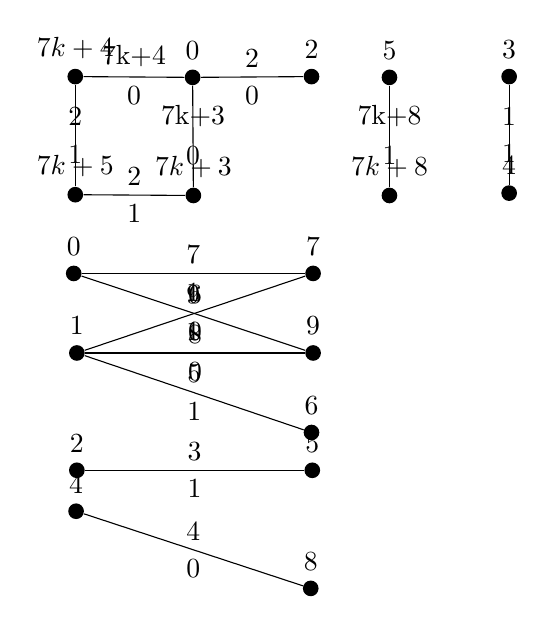
\begin{tikzpicture}
\node[fill=black, circle, inner sep=2pt, label=above:{\textcolor{black}{${2}$} }] (Graph with 9 nodes and 7 edgesN2) at (5.5,-0.49) {};
\node[fill=black, circle, inner sep=2pt, label=above:{\textcolor{black}{${0}$} }] (Graph with 9 nodes and 7 edgesN0) at (3.99,-0.5) {};
\node[fill=black, circle, inner sep=2pt, label=above:{\textcolor{black}{${7k+3}$} }] (Graph with 9 nodes and 7 edgesN7k+3) at (4.0,-2.0) {};
\node[fill=black, circle, inner sep=2pt, label=above:{\textcolor{black}{${7k+5}$} }] (Graph with 9 nodes and 7 edgesN7k+5) at (2.5,-1.99) {};
\node[fill=black, circle, inner sep=2pt, label=above:{\textcolor{black}{${7k+4}$} }] (Graph with 9 nodes and 7 edgesN7k+4) at (2.5,-0.49) {};
\node[fill=black, circle, inner sep=2pt, label=above:{\textcolor{black}{${7k+8}$} }] (Graph with 9 nodes and 7 edgesN7k+8) at (6.49,-2.0) {};
\node[fill=black, circle, inner sep=2pt, label=above:{\textcolor{black}{${3}$} }] (Graph with 9 nodes and 7 edgesN3) at (8.01,-0.49) {};
\node[fill=black, circle, inner sep=2pt, label=above:{\textcolor{black}{${4}$} }] (Graph with 9 nodes and 7 edgesN4) at (8.01,-1.97) {};
\node[fill=black, circle, inner sep=2pt, label=above:{\textcolor{black}{${5}$} }] (Graph with 9 nodes and 7 edgesN5) at (6.49,-0.5) {};
\draw[draw=black, shorten >=3pt, shorten <=3pt] (3.99,-0.5) -- (4.0,-2.0);
\node[above, text=black] at (3.995,-1.25) {\textcolor{black}{7k+3}};
\node[below, text=black] at (3.995,-1.25) {\textcolor{black}{0}};
\draw[draw=black, shorten >=3pt, shorten <=3pt] (3.99,-0.5) -- (2.5,-0.49);
\node[above, text=black] at (3.245,-0.495) {\textcolor{black}{7k+4}};
\node[below, text=black] at (3.245,-0.495) {\textcolor{black}{0}};
\draw[draw=black, shorten >=3pt, shorten <=3pt] (3.99,-0.5) -- (5.5,-0.49);
\node[above, text=black] at (4.745,-0.495) {\textcolor{black}{2}};
\node[below, text=black] at (4.745,-0.495) {\textcolor{black}{0}};
\draw[draw=black, shorten >=3pt, shorten <=3pt] (4.0,-2.0) -- (2.5,-1.99);
\node[above, text=black] at (3.25,-1.995) {\textcolor{black}{2}};
\node[below, text=black] at (3.25,-1.995) {\textcolor{black}{1}};
\draw[draw=black, shorten >=3pt, shorten <=3pt] (2.5,-1.99) -- (2.5,-0.49);
\node[above, text=black] at (2.5,-1.24) {\textcolor{black}{2}};
\node[below, text=black] at (2.5,-1.24) {\textcolor{black}{1}};
\draw[draw=black, shorten >=3pt, shorten <=3pt] (8.01,-0.49) -- (8.01,-1.97);
\node[above, text=black] at (8.01,-1.23) {\textcolor{black}{1}};
\node[below, text=black] at (8.01,-1.23) {\textcolor{black}{1}};
\draw[draw=black, shorten >=3pt, shorten <=3pt] (6.49,-0.5) -- (6.49,-2.0);
\node[above, text=black] at (6.49,-1.25) {\textcolor{black}{7k+8}};
\node[below, text=black] at (6.49,-1.25) {\textcolor{black}{1}};
\node[fill=black, circle, inner sep=2pt, label=above:{\textcolor{black}{${0}$} }] (Graph with 9 nodes and 7 edgesN0) at (2.48,-2.99) {};
\node[fill=black, circle, inner sep=2pt, label=above:{\textcolor{black}{${7}$} }] (Graph with 9 nodes and 7 edgesN7) at (5.52,-2.99) {};
\node[fill=black, circle, inner sep=2pt, label=above:{\textcolor{black}{${1}$} }] (Graph with 9 nodes and 7 edgesN1) at (2.52,-4.0) {};
\node[fill=black, circle, inner sep=2pt, label=above:{\textcolor{black}{${6}$} }] (Graph with 9 nodes and 7 edgesN6) at (5.5,-5.01) {};
\node[fill=black, circle, inner sep=2pt, label=above:{\textcolor{black}{${9}$} }] (Graph with 9 nodes and 7 edgesN9) at (5.52,-4.0) {};
\node[fill=black, circle, inner sep=2pt, label=above:{\textcolor{black}{${8}$} }] (Graph with 9 nodes and 7 edgesN8) at (5.49,-6.99) {};
\node[fill=black, circle, inner sep=2pt, label=above:{\textcolor{black}{${2}$} }] (Graph with 9 nodes and 7 edgesN2) at (2.52,-5.49) {};
\node[fill=black, circle, inner sep=2pt, label=above:{\textcolor{black}{${4}$} }] (Graph with 9 nodes and 7 edgesN4) at (2.51,-6.01) {};
\node[fill=black, circle, inner sep=2pt, label=above:{\textcolor{black}{${5}$} }] (Graph with 9 nodes and 7 edgesN5) at (5.51,-5.49) {};
\draw[draw=black, shorten >=3pt, shorten <=3pt] (2.48,-2.99) -- (5.52,-2.99);
\node[above, text=black] at (4.0,-2.99) {\textcolor{black}{7}};
\node[below, text=black] at (4.0,-2.99) {\textcolor{black}{1}};
\draw[draw=black, shorten >=3pt, shorten <=3pt] (2.48,-2.99) -- (5.52,-4.0);
\node[above, text=black] at (4.0,-3.495) {\textcolor{black}{9}};
\node[below, text=black] at (4.0,-3.495) {\textcolor{black}{1}};
\draw[draw=black, shorten >=3pt, shorten <=3pt] (5.52,-2.99) -- (2.52,-4.0);
\node[above, text=black] at (4.02,-3.495) {\textcolor{black}{6}};
\node[below, text=black] at (4.02,-3.495) {\textcolor{black}{0}};
\draw[draw=black, shorten >=3pt, shorten <=3pt] (2.52,-4.0) -- (5.52,-4.0);
\node[above, text=black] at (4.02,-4.0) {\textcolor{black}{8}};
\node[below, text=black] at (4.02,-4.0) {\textcolor{black}{0}};
\draw[draw=black, shorten >=3pt, shorten <=3pt] (2.52,-4.0) -- (5.5,-5.01);
\node[above, text=black] at (4.01,-4.505) {\textcolor{black}{5}};
\node[below, text=black] at (4.01,-4.505) {\textcolor{black}{1}};
\draw[draw=black, shorten >=3pt, shorten <=3pt] (2.51,-6.01) -- (5.49,-6.99);
\node[above, text=black] at (4.0,-6.5) {\textcolor{black}{4}};
\node[below, text=black] at (4.0,-6.5) {\textcolor{black}{0}};
\draw[draw=black, shorten >=3pt, shorten <=3pt] (2.52,-5.49) -- (5.51,-5.49);
\node[above, text=black] at (4.015,-5.49) {\textcolor{black}{3}};
\node[below, text=black] at (4.015,-5.49) {\textcolor{black}{1}};
\end{tikzpicture}
\end{document}
